% Общий объем раздела 25-30 стр.

\section{Разработка и реализация алгоритмов стегоанализа изображений с использованием свёрточных искусственных нейронных сетей}

Широкое распространение стегоаналитических подходов, использующих МОВ, дало мощный толчок для построения стеганографических систем с большей стегоскрытностью, что в свою очередь дало старт росту размерности пространства признаков, формируемого стегоаналитиком. Ручное конструирование сотен признаков --- трудоёмкая задача, что стало одной из причин появления стегоаналитических алгоритмов с использованием свёрточных искусственных нейронных сетей.

\subsection{Описание нейросетевого подхода и общей схемы алгоритма}



\subsection{Возможные архитектуры и параметры используемых нейронных сетей}

\subsubsection{Свёрточная нейронная сеть GNCNN}

Модель свёрточной нейронной сети для стегоанализа изображений в оттенках серого GNCNN была предложена в~\cite{GNCNN}. Её основные отличительные особенности: применение фильтра предварительной обработки и использование функции Гаусса в качестве функции активации нейронов свёрточных слоёв.
\begin{equation}
\label{eq:GNCNNConvKernel}
%\begin{align*}
K = \frac{1}{12}
\begin{pmatrix*}[r]
    -1 &  2 &    -2 &  2 & -1 \\
     2 & -6 &     8 & -6 &  2 \\
    -2 &  8 & -12 &  8 & -2 \\
     2 & -6 &     8 & -6 &  2 \\
    -1 &  2 &    -2 &  2 & -1 \\
\end{pmatrix*}
%\end{align*}
\end{equation}

Полосовой высокочастотный фильтр предварительной обработки с импульсной характеристикой~\eqref{eq:GNCNNConvKernel} введён исходя из априорного знания о слабом характере стеговоздействия на стегоконтейнер. Целью предварительной фильтрации является усиление яркости стегосигнала и ослабление яркости оригинального изображения. Веса данного фильтра заранее предопределены и не участвуют в процессе обучения нейронной сети.

Ещё одним преобразованием, облегчающим процесс извлечения признаков, является переход от оригинального изображения к шумоподобному остатку $ R = (r_{ij}) $, содержащему только предсказания относительно факта стеганографической модификации каждого пикселя:
\begin{equation*}
r_{ij} = y_{ij} - P(N(Y, i, j)),
\end{equation*}
где $ Y = (y_{ij}) $ – стегоконтейнер, а $ P(N(Y, i, j)) $ – оценка значения пикселя $ y_{ij} $, полученная из окружающих его пикселей $ N(Y, i, j) $~\cite{FridrichNoiseResidual}. Ввиду наличия сложных зависимостей между соседними пикселями, в случае отсутствия модификации оценка зачастую будет близка к действительному значению пикселя $ y_{ij} $, а значение $ r_{ij} $ будет близко к нулю.
\begin{equation}
\label{eq:GaussianFunction}
%\begin{align*}
f(x) = e^{-\frac{x^2}{\sigma^2}}
%\end{align*}
\end{equation}

Функция Гаусса~\eqref{eq:GaussianFunction} с нулевым математическим ожиданием в качестве функции активации (рис.~\ref{fig:GaussianFunction}) призвана обеспечить формирование в свёрточном слое нейронной сети такого ядра $ K $, что $ Y*K = R $. Максимальное значение функции в нуле соответствует нулевой ошибке оценки значения $ y_{ij} $ и, следовательно, предположению об отсутствии модификации пикселя стегоконтейнера. Резкий спад по мере удаления от нуля обращает в близкие к нулю значения любой результат свёртки, превышающий порог, определяемый среднеквадратическим отклонением $ \sigma $, влияющим на ширину кривой. В рамках эксперимента использовалось значение $ \sigma = 0,1 $.

\begin{figure}
\centering
\includegraphics[width=1\textwidth]{include/graphics/gaussian_function}
\caption{Функция активации GNCNN}
\label{fig:GaussianFunction}
\end{figure}

В процессе обучения в качестве функции потерь применялась категориальная кросс-энтропия. Используемый метод обучения – Adam со скоростью обучения 0,001, $ \beta_1 = 0,9 $, $ \beta_2 = 0,999 $. Архитектура нейронной сети представлена на рис.~\ref{fig:GNCNNArchitecture} и имеет вид состояний, через которые проходит входное изображение.

\begin{figure}
\centering
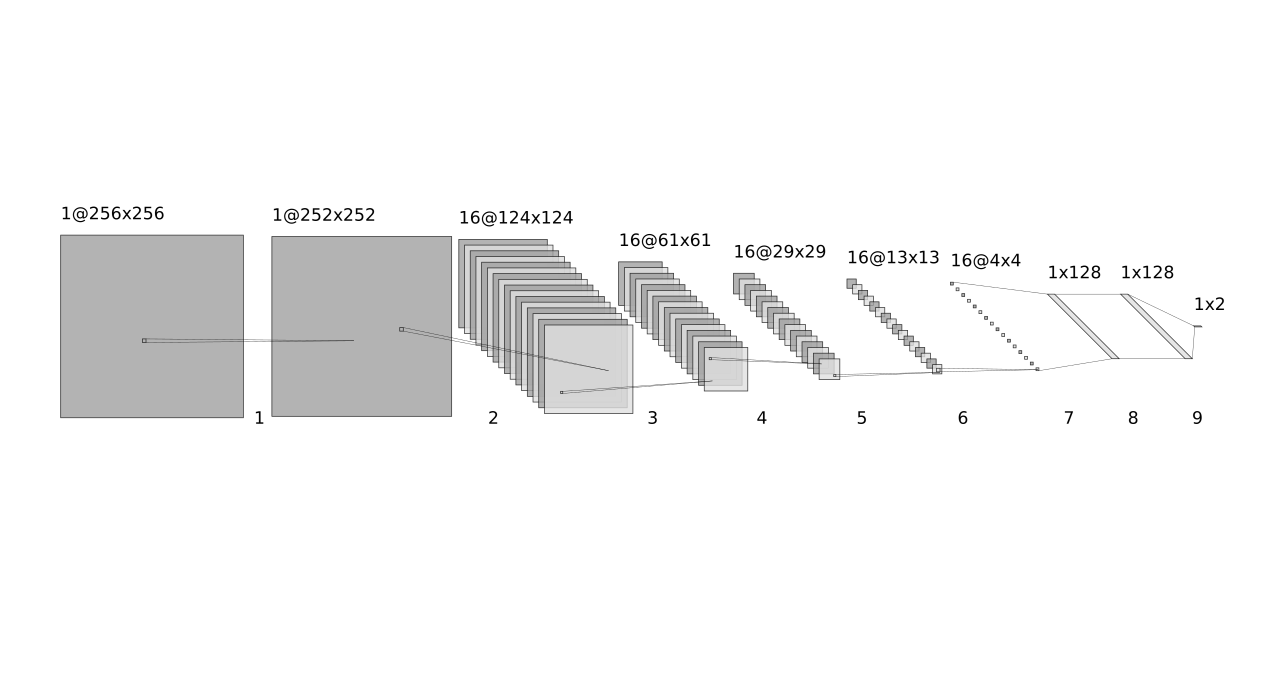
\includegraphics[width=1\textwidth]{include/graphics/gncnn_gray_architecture}
\caption{Архитектура GNCNN}
\label{fig:GNCNNArchitecture}
\end{figure}

На вход нейронной сети подаётся изображение в оттенках серого в разрешении 256×256 пикселей. Фильтр предварительной обработки с ядром~\eqref{eq:GNCNNConvKernel} является первым свёрточным слоем и в обучении не участвует. За ним следуют пять свёрточных слоёв, состоящих из 16 каналов. Каждый из них осуществляет операцию свёртки с ядром, формирующимся по мере обучения сети, а также вычисление функции активации и выполнение субдискретизации по среднему с размером окна 3×3 и шагом 2. Первые четыре обучаемых слоя используют ядра размера 3×3, последний – 5×5.

Выход последнего свёрточного слоя представляет собой 256 выделенных признака. Они помещаются в модуль классификации, состоящий из трёх полносвязных слоёв: первые два имеют по 128 нейронов каждый и функцию активации ReLU, последний – два нейрона и функцию активации softmax.

\subsubsection{Нейронная сеть с двумя свёрточными слоями}
Также в рамках работы была рассмотрена свёрточная нейронная сеть для стегоанализа изображений в оттенках серого, предложенная в~\cite{FrenchCNN}. Для корректности эксперимента размеры слоёв были изменены для работы со входными изображениями в разрешении 256×256 пикселей. Архитектура нейронной сети приведена на~\ref{fig:FrenchCNNArchitecture}.

% Рисунок 1.4 -- French CNN Architecture
\begin{figure}[!htb]
\centering
\includegraphics[width=1\textwidth]{include/graphics/french_gray_architecture}
\caption{Архитектура сети с двумя свёрточными слоями}
\label{fig:FrenchCNNArchitecture}
\end{figure}

На вход нейронной сети подаётся изображение в оттенках серого в разрешении 256×256 пикселей. Первый свёрточный слой имеет размер 3×3, за ним следует свёрточный слой размера 253×253, состоящий из 64 каналов. Оба свёрточных слоя осуществляют операцию свёртки с обучаемым ядром и вычисление функции активации tanh. Результатом их работы являются 64 карты признаков размера 2×2, соединённые с двумя нейронами с функцией активации softmax.

В качестве функции потерь была использована категориальная кросс-энтропия, метод обучения – стохастический градиентный спуск со скоростью обучения 0,005.
\subsection{Алгоритмы предобработки данных при проведении стегоанализа}

\clearpage
